\section{Context and Scope}

Since this system relies on the correct working of external elements it is important that their interaction is 
corrected displayed.

\subsection{Business Context}

\begin{figure}[H]
    \centering
    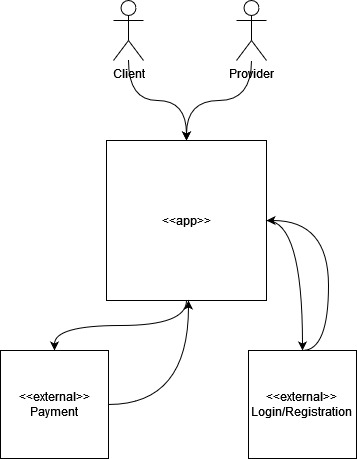
\includegraphics[width=0.5\textwidth]{assets/business_context.jpg}
    \caption{Preliminary functions}
    \label{fig:business_context}
\end{figure}

\begin{table}[H]
    \setstretch{1.0}
    \begin{tabularx}{\textwidth}{lX}
    \toprule
    ID & Description   \\
    \midrule
    \gls{client} & Searches for a last time offer from a restaurant, bakery or pastry. \\
    \gls{provider} & Offers a still consumable product that was not sold during normal working time. \\
    Payment & Deals with the payment processing using registered information from another payment platforms. \\
    Login/Registration & Authenticated \glsplural{user} using logins from other platforms.  \\
    \bottomrule
    \end{tabularx}
\end{table}

\subsection{Technical Context}

\begin{figure}[H]
    \centering
    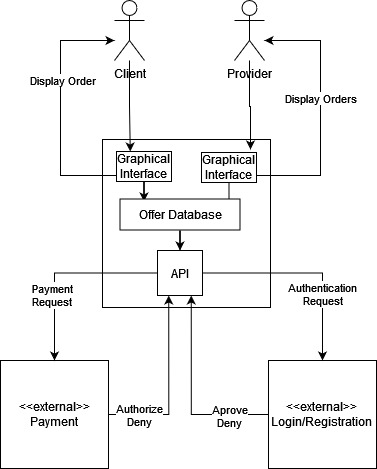
\includegraphics[width=0.5\textwidth]{assets/technical_context.jpg}
    \caption{Preliminary functions}
    \label{fig:technical_context}
\end{figure}

\begin{table}[H]
    \setstretch{1.0}
    \begin{tabularx}{\textwidth}{lX}
    \toprule
    ID & Description   \\
    \midrule
    \gls{client} & AAAAAAAAAAAAAAAAAAAAAAAA \\
    \gls{provider} & AAAAAAAAAAAAAAAAAAAAAAAAAA \\
    Payment & AAAAAAAAAAAAAAAAA \\
    Login/Registration & AAAAAAAAAAAA  \\
    \bottomrule
    \end{tabularx}
\end{table}